\documentclass[11p,aspectratio=169]{beamer}

\geometry{paperwidth=160mm,paperheight=120mm}

\usetheme[{titleformat plain}=smallcaps,
           titleformat title=smallcaps,
           titleformat subtitle=regular,
           titleformat section=smallcaps,
           titleformat frame=smallcaps,
        %    numbering=fraction,
          ]{metropolis}

\usepackage{style/main}
\usepackage[T1]{fontenc}
\usepackage[english]{babel}
\usepackage{graphicx}
\usepackage{tcolorbox}
\usepackage{xcolor}
\usepackage{amsmath,bm,amsfonts,amssymb,array,calc,amsthm,rotating,amscd,bbm}
\usepackage{url}
\usepackage{minted}
\usepackage{hyperref}
\usepackage{fontawesome}
\usepackage{movie15}
\usepackage{tikz}
\usepackage{multicol}
\usepackage{wrapfig}
\usetikzlibrary{quantikz}
\setbeamercolor{background canvas}{bg=white}
% in documenet


\usefonttheme[onlymath]{serif}
\usepackage[absolute,overlay]{textpos}

\setbeamerfont{caption}{size=\scriptsize}
% \usepackage[natbib=true,backend=biber,useprefix=true]{biblatex}
% \addbibresource{references.bib}
% \setbeamercolor{bibliography item}{parent=palette primary}
% \setbeamercolor*{bibliography entry title}{parent=palette primary}

% \usetheme[progressbar=frametitle]{metropolis}
% \setbeamertemplate{frame numbering}[fraction]
% \metroset{background=dark}
% \definecolor{primary}{RGB}{245, 10, 10}
% \setbeamercolor{palette primary}{bg=white, fg=black}
% \setbeamercolor{background canvas}{parent=palette primary}
% \setbeamercolor{normal text}{fg=black}
% \setbeamercolor{progress bar}{use=palette primary, fg=primary}
% natbib=true,style=authoryear,backend=bibtex,useprefix=true
% \setbeamerfont{caption}{size=\tiny}

% \usepackage[style=authoryear]{biblatex}
%%% THIS ADDS THE COMMA BETWEEN AUTHOR NAME AND YEAR
% \renewcommand*{\nameyeardelim}{\addcomma\space}
% \addbibresource{test.bib}


% \title{Towards a hybrid quantum operating system}
% \subtitle{First Year PhD students workshop}
% \author{Andrea Pasquale}
% \date{30th September 2022}
% \titlegraphic{
%     \vspace*{11.5cm}
%     \raisebox{20pt}[10pt][10pt]{
\includegraphics[height=4cm]{../logos/unimi_logo.pdf}}\hspace*{30pt}
%     \raisebox{20pt}[10pt][10pt]{
\includegraphics[height=4cm]{../logos/tii_logo.png}}\hspace*{30pt}
%     \raisebox{20pt}[10pt][10pt]{
\includegraphics[height=4cm]{../logos/infn_logo.png}}\hspace*{30pt}
%     % \includegraphics[height=1.3cm]{../_logos/erc_logo1.png}

%     % \vfill\vspace*{230pt}
%     % 
\includegraphics[height=1cm]{../_logos/unimi_logo.png}\hfill
%     % 
\includegraphics[height=1cm]{../_logos/infn_logo.png}\\
%     % \vspace*{5pt}
%     % {
%     %     \fontsize{3pt}{3.5pt}\selectfont
%     %     \begin{center}
%     %         This project has received funding from the European Union's Horizon
%     %         2020 research and innovation programme under grant agreement No
%     %         % 740006\quad \includegraphics[height=5pt]{../_logos/eu-flag.jpg}
%     %     \end{center}
%     % }
% }


\begin{document}

% \maketitle

\begin{frame}{What is Qibo?}
    Qibo is an \textbf{open-source} full stack API for quantum simulation and quantum hardware control and calibration.
    \begin{figure}
        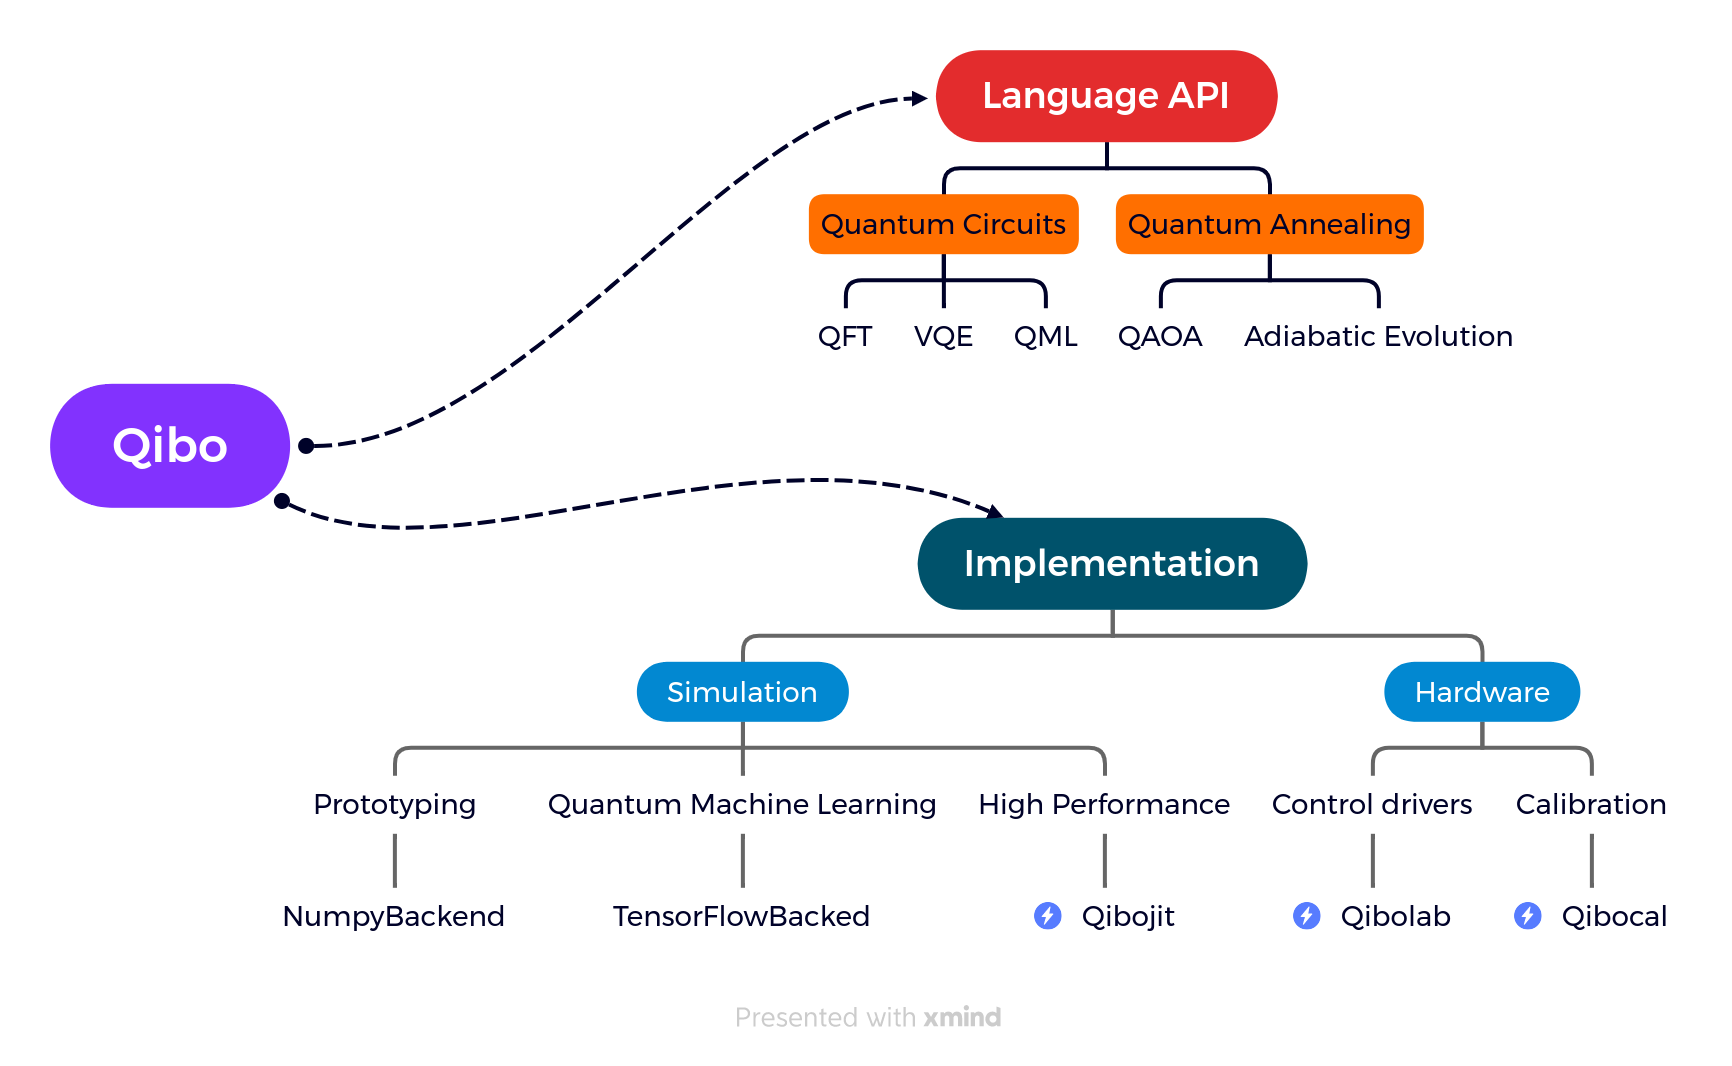
\includegraphics[width= \textwidth]{figures/Qibo.png}
    \end{figure}
\end{frame}

\begin{frame}{Motivation}
    We are developing a new tool called {\color{blue} \textbf{Qibocal}} to perform qubits calibration in Qibo using Qibolab as the main driver.
    
    The main features that we are implemented are the following:


    \begin{multicols*}{2}
        \begin{itemize}
            \item[\faCaretSquareORight] Platform agnostic approach
            \item[\faCaretSquareORight] Launch calibration routines easily
            \item[\faCaretSquareORight] Live-plotting tools
            \item[\faCaretSquareORight] Live-fitting tools
            \item[\faCaretSquareORight] Save and share your data
            \item[\faCaretSquareORight] Autocalibration
        \end{itemize}
    \end{multicols*}
\end{frame}

\begin{frame}{Qibocal: implementation}
    \begin{figure}
        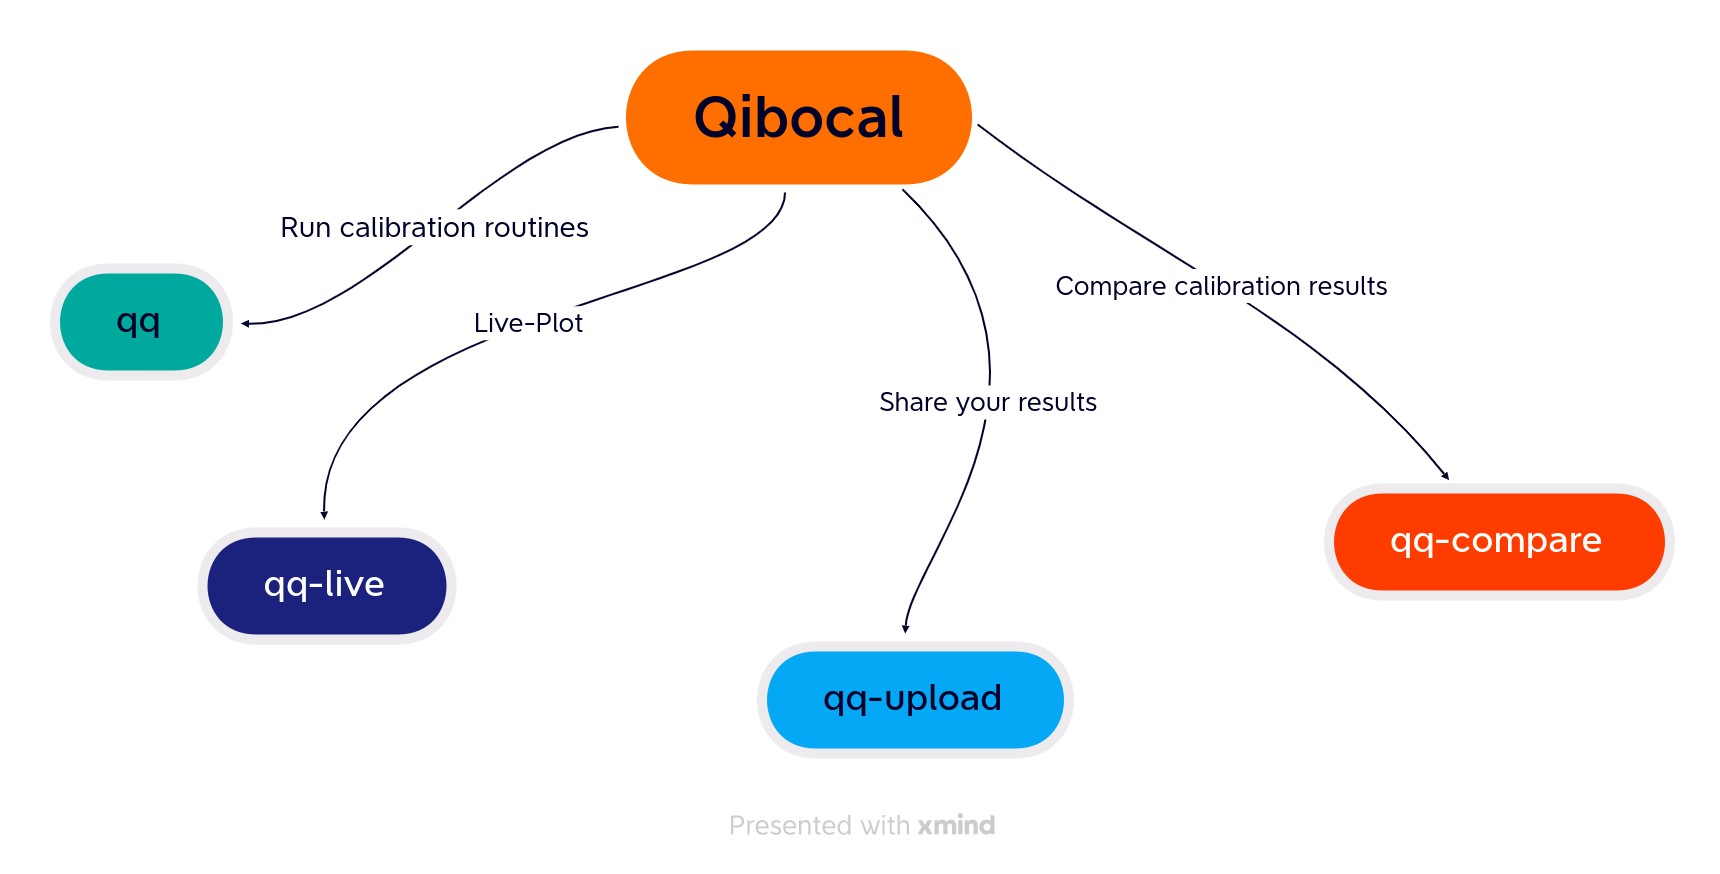
\includegraphics[width= \textwidth]{figures/Qibocal.png}
    \end{figure}
\end{frame}

\begin{frame}{Single Qubit characterization}
    \begin{figure}
        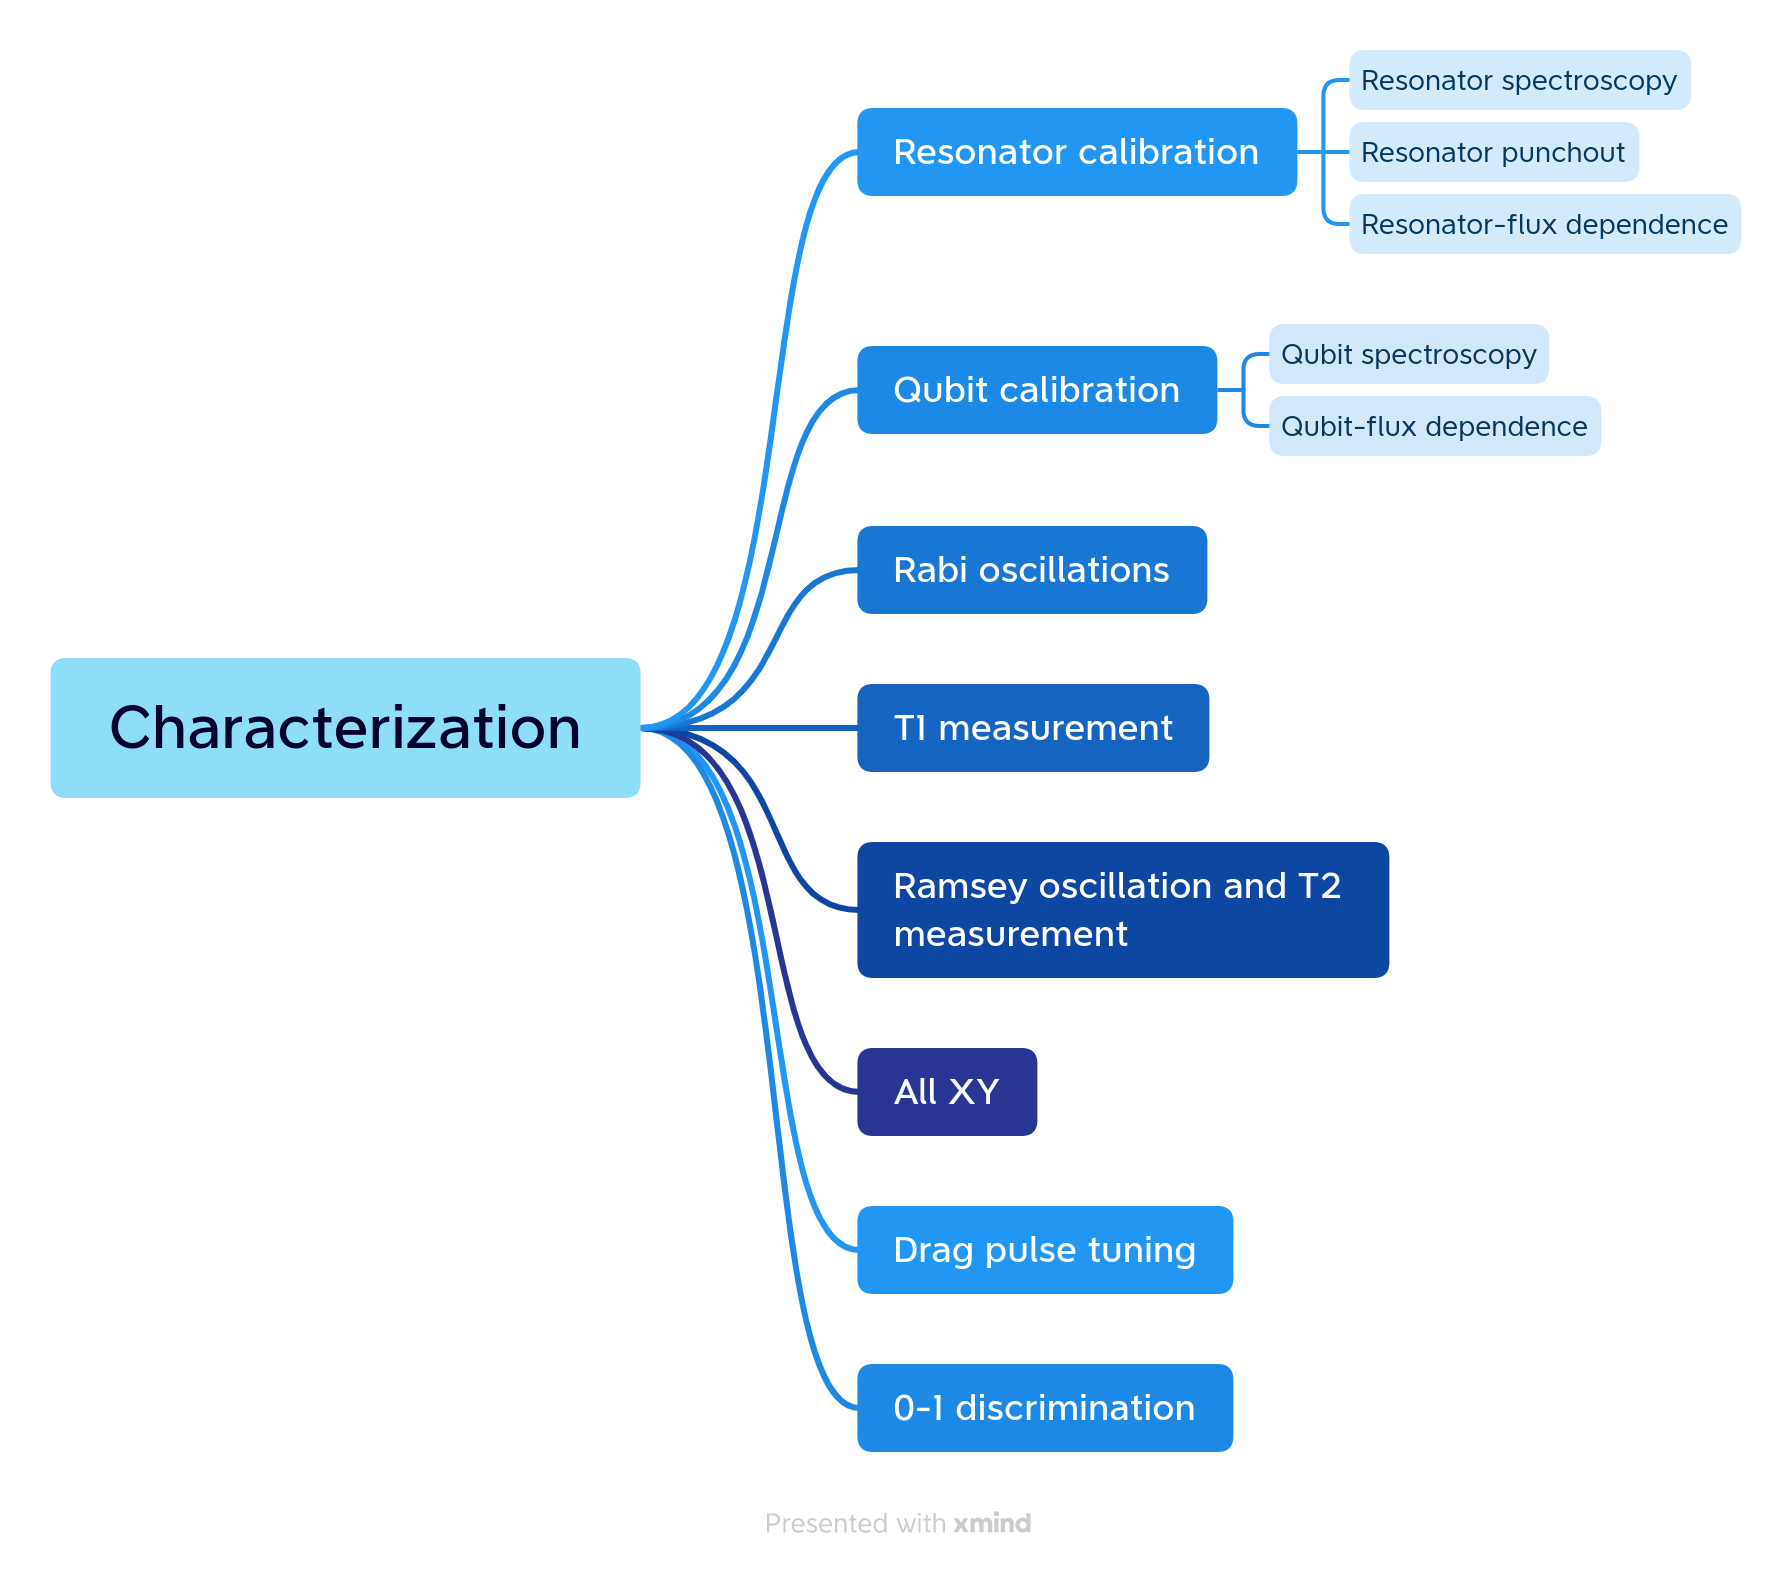
\includegraphics[width= 0.8 \textwidth]{figures/Characterization.png}
    \end{figure}
\end{frame}

\begin{frame}{Extract fidellity using quantum protocols}
    We are also looking to include various quantum protocols to extract the fidelity
    \begin{figure}
        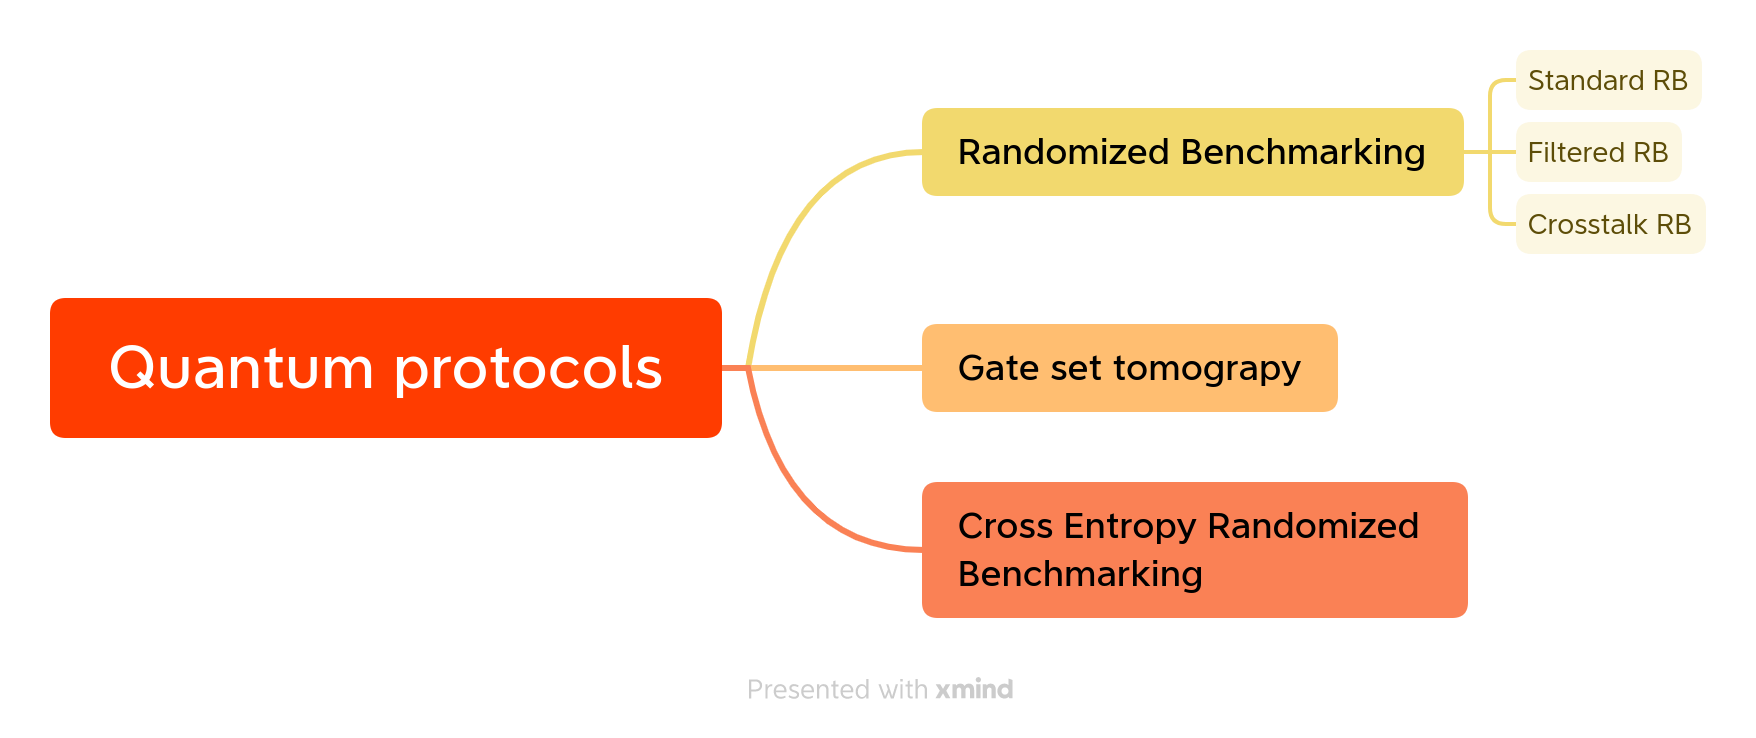
\includegraphics[width= 0.8 \textwidth]{figures/Quantum protocols.png}
    \end{figure}
\end{frame}

\begin{frame}{How to use \texttt{qq}}
    To run a specific set of calibration it is sufficient to write a runcard:
    \begin{multicols*}{2}
        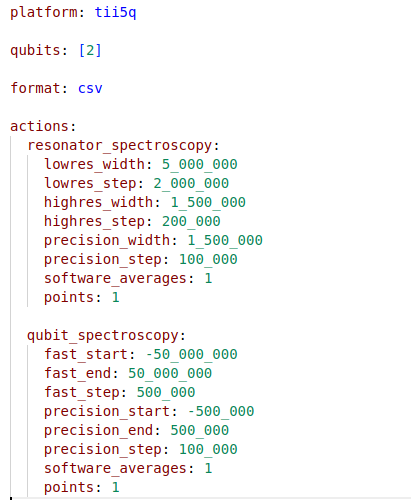
\includegraphics[width= 0.5 \textwidth]{figures/runcard.png}
        You can execute the following runcard by typing:
        \begin{center}
            \texttt{qq} \texttt{<runcard.yaml>} 
        \end{center}

    \texttt{qq} will take care of:
    \begin{itemize}
        \item connecting to the platform
        \item executing the routines listed under actions
        \item generating an update runcard for the platform
        \item generating a web report containing the results
    \end{itemize}
    \end{multicols*}
    \
\end{frame}

\begin{frame}{How to use \texttt{qq-live}}
    Using \texttt{qq-live} it is possible to visualize the results during (after) the execution
    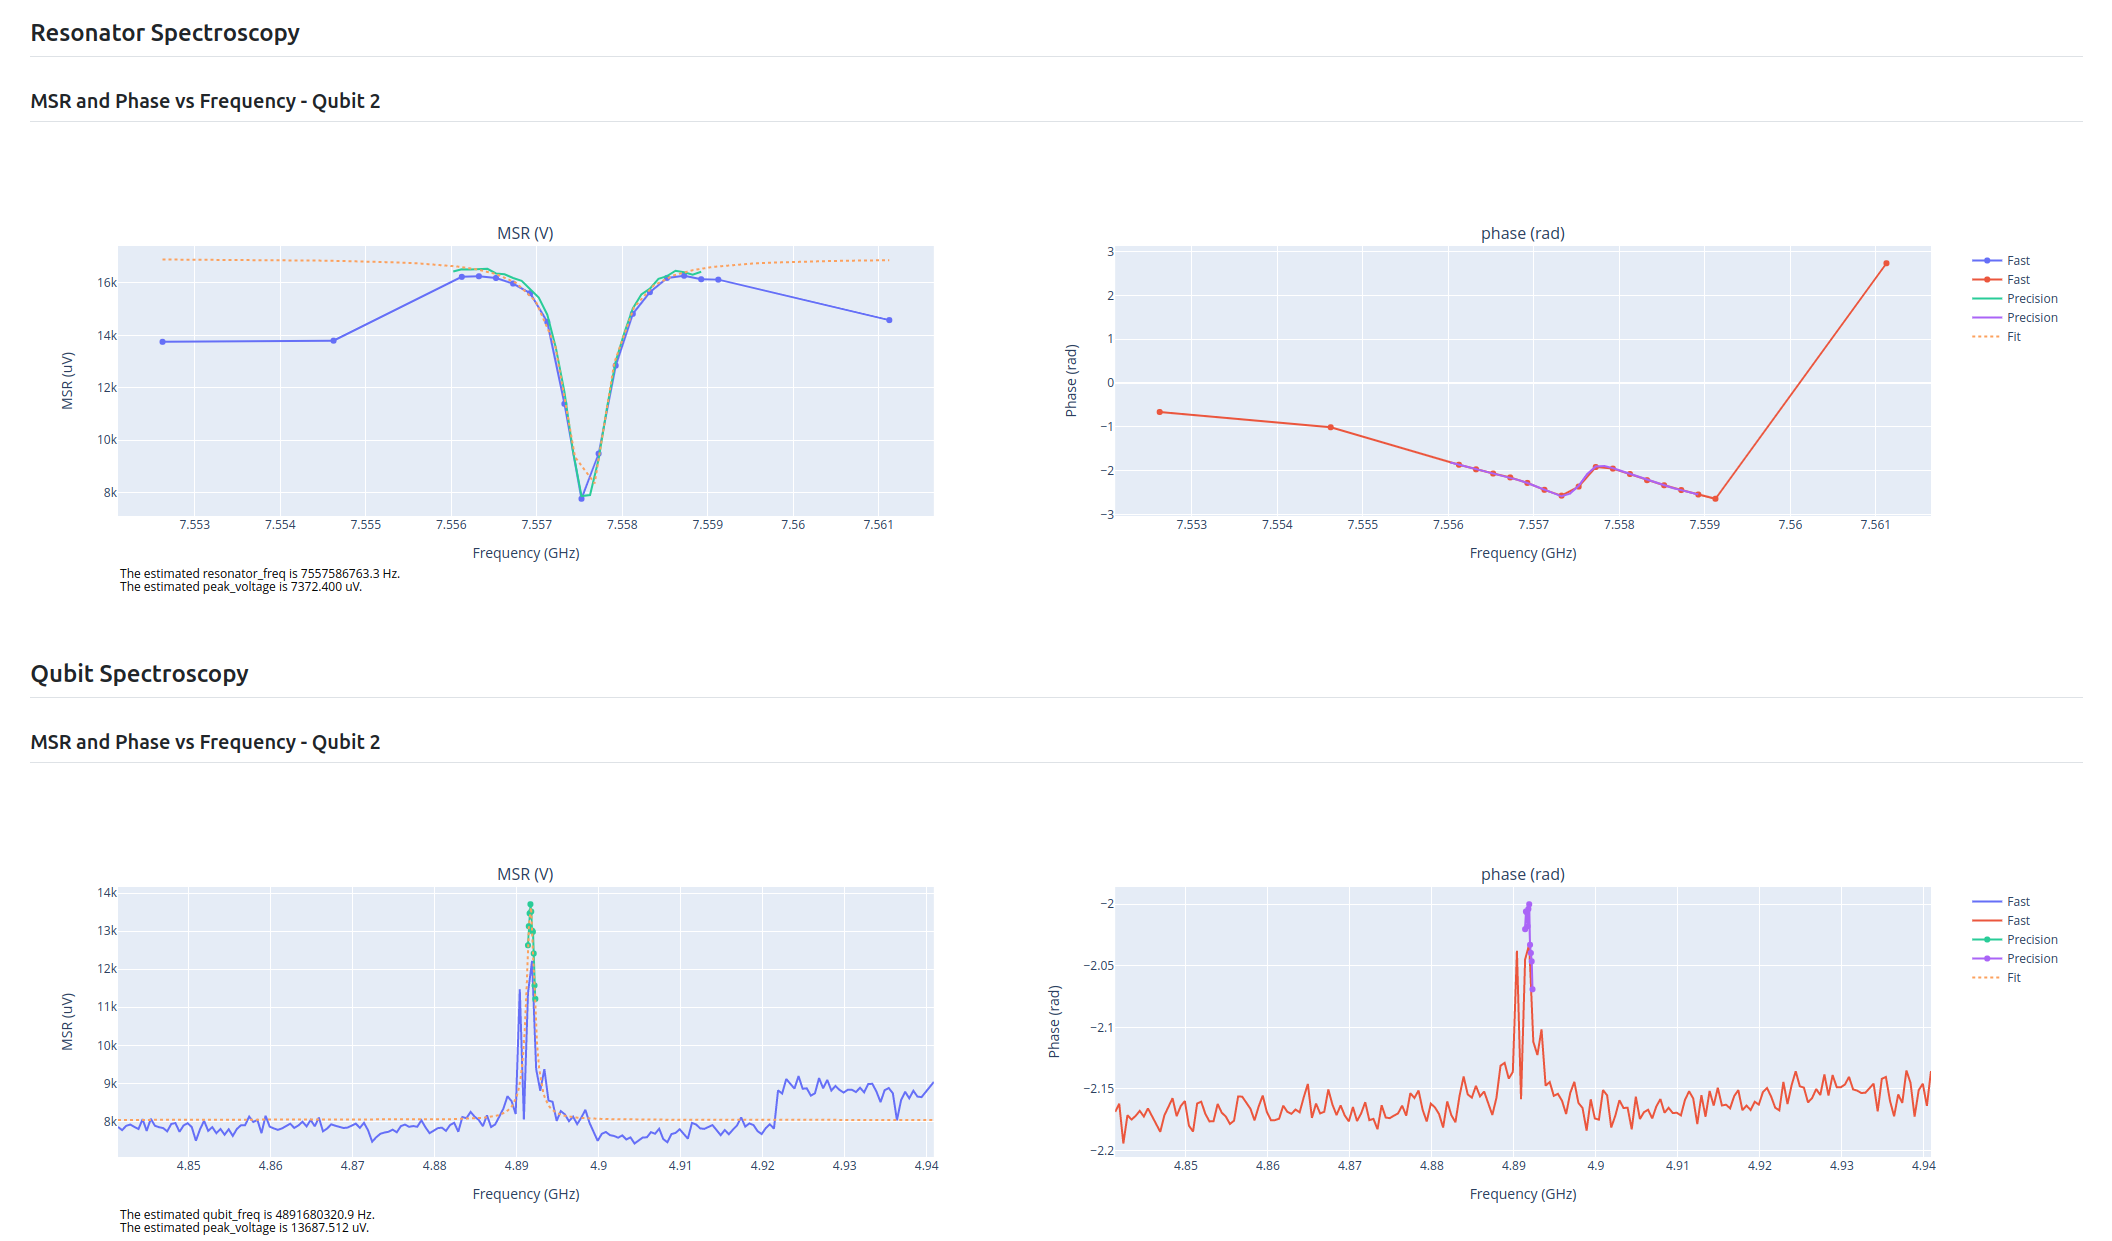
\includegraphics[width=\textwidth]{figures/qq-live.png}
\end{frame}

\begin{frame}{How to use \texttt{qq-upload}}
    
    You can share your results by uploading the report generated by \texttt{qq} using \texttt{qq-upload}
    \vspace{0.3cm}
    
    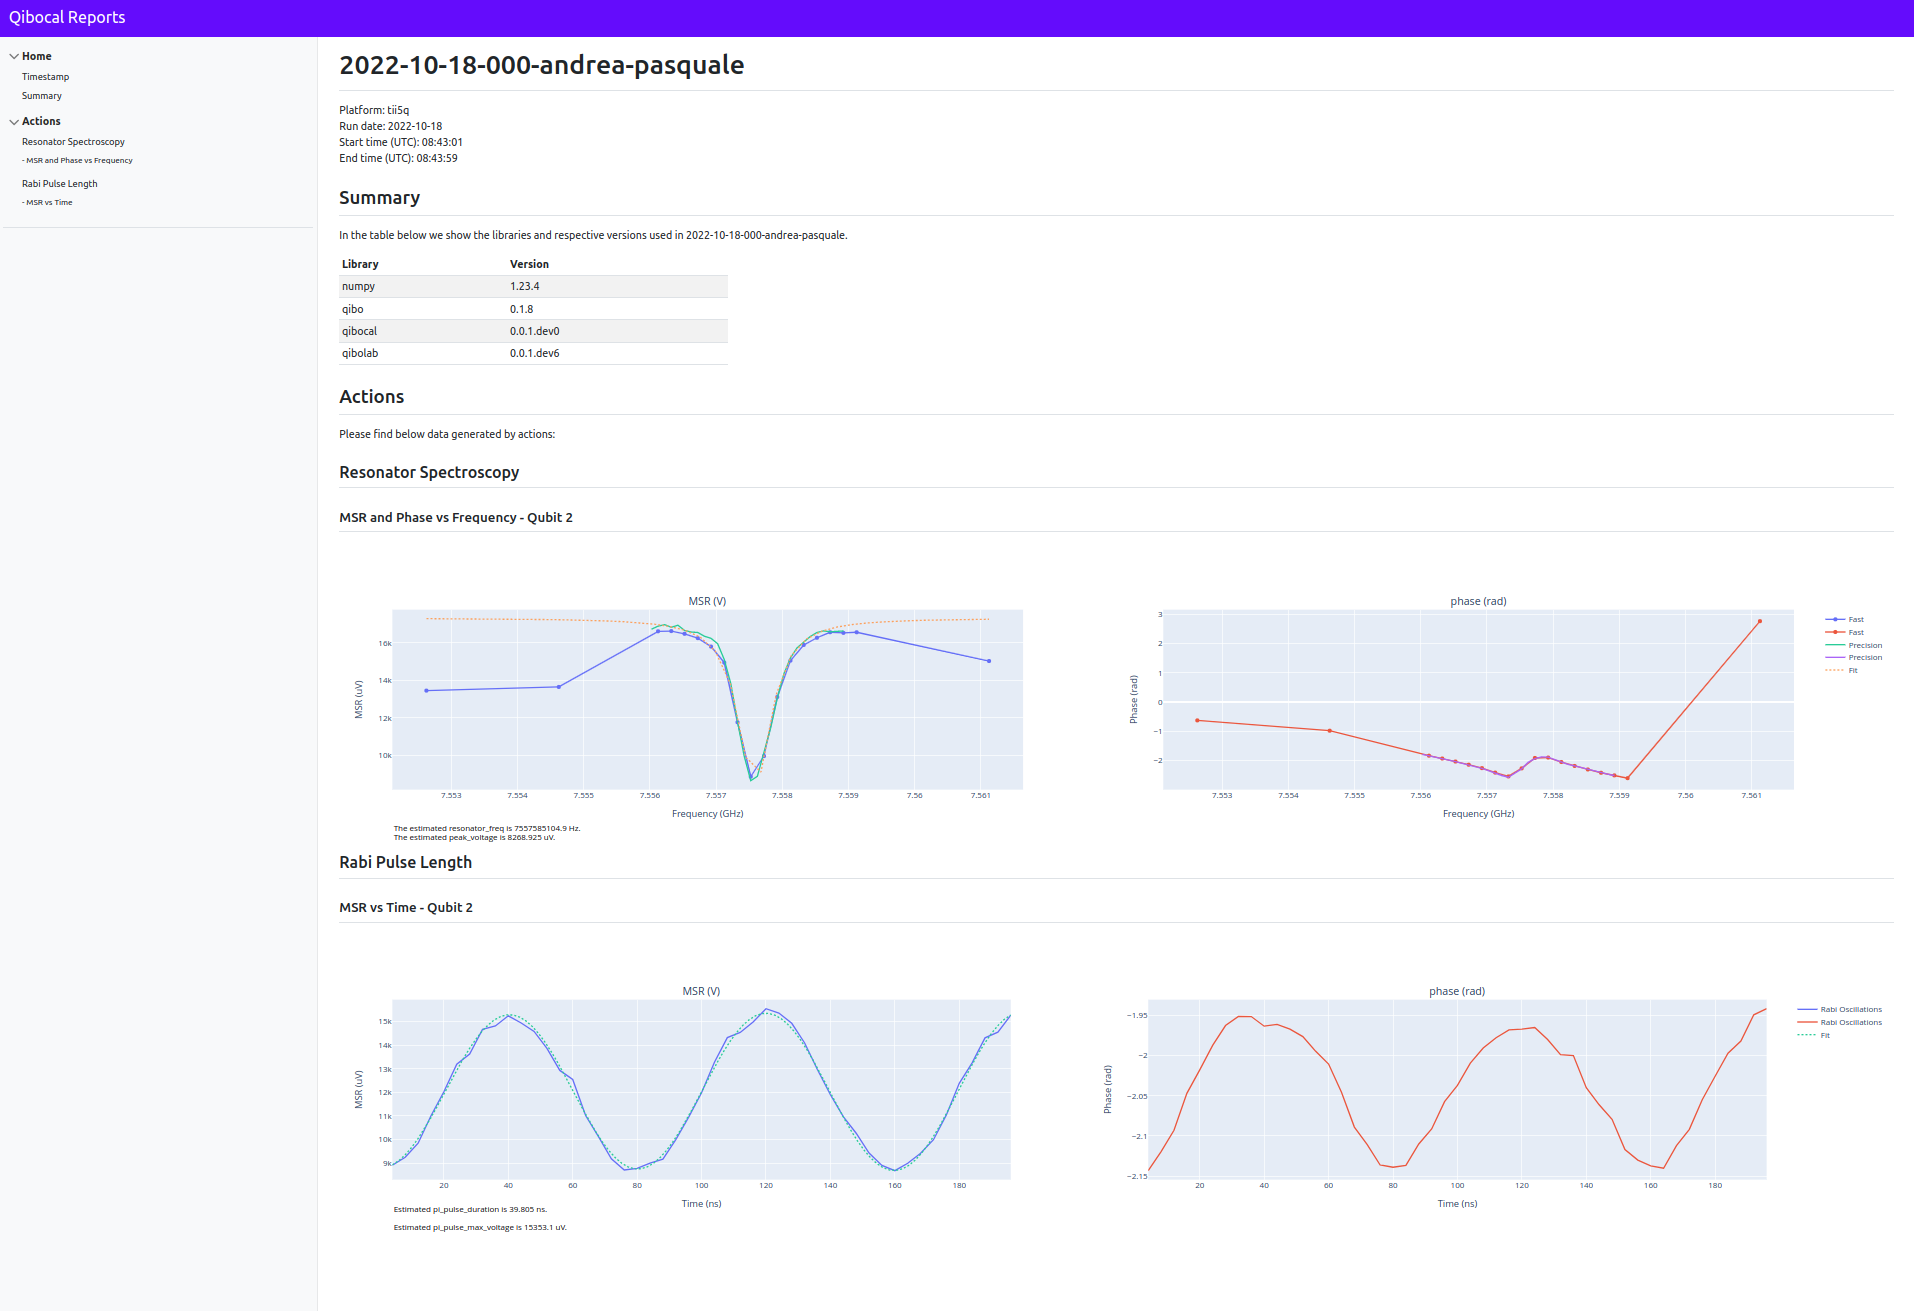
\includegraphics[width=\textwidth]{figures/upload.png}
\end{frame}
\end{document}